\documentclass[11pt]{article}
\usepackage[margin=1in]{geometry}
\usepackage{amsmath, amssymb, mathtools}
\usepackage{lmodern}
\usepackage[T1]{fontenc}
\usepackage{microtype}
\usepackage{url}
\usepackage{breakurl}
\usepackage{booktabs}
\usepackage{graphicx}
\usepackage{float}
\usepackage{adjustbox}

\title{Problem Set \#5}
\author{Marli Fichtner}
\date{October 7, 2025}

\begin{document}
\maketitle

\begin{itemize}
\item 
    \textbf{Research Question:} Are there differences in developmental screening rates across states or insurance types?

\item 
    \textbf{Data Source:} 2016-2020 National Survey of Children's Health (NSCH). Due to the federal government shutdown, data for 2018 was not collected, and this was omitted from the analysis.

    \item
\textbf{Context:} The National Survey of Children's Health (NSCH) provides data on various aspects of children's health and well-being, including developmental screening rates. In December 2016, the American Academy of Pediatrics (AAP) and the Centers for Disease Control and Prevention (CDC) released updated guidelines recommending that all children aged 9, 18, and 30 months receive developmental screenings during their well-child visits.

This study aims to analyze the NSCH data to identify any disparities in developmental screening rates based on state of residence and type of health insurance coverage. The study will include a basic linear regression model, with the following specifications:

Secondly, the study will explore potential interaction effects between state and insurance type to determine if the relationship between insurance type and developmental screening rates varies by state. This specification will help to uncover more nuanced patterns in the data and provide insights into how different factors may jointly influence developmental screening rates. The identifying equation will include state fixed effects and insurance type indicators.

Thirdly, the study will utilize a regression discontinuity design to quantify the impact of the implementation of the new AAP guidelines in January 2017 on developmental screening rates, by state.

\textbf{Independent Variables:} State, Insurance Type

\textbf{Dependent Variables:} Developmental Screening Rates (4.10 Developmental screening, 9-35 months (NPM-6))

\end{itemize}
\subsection{Visualizations}

\begin{figure}[H]
\centering
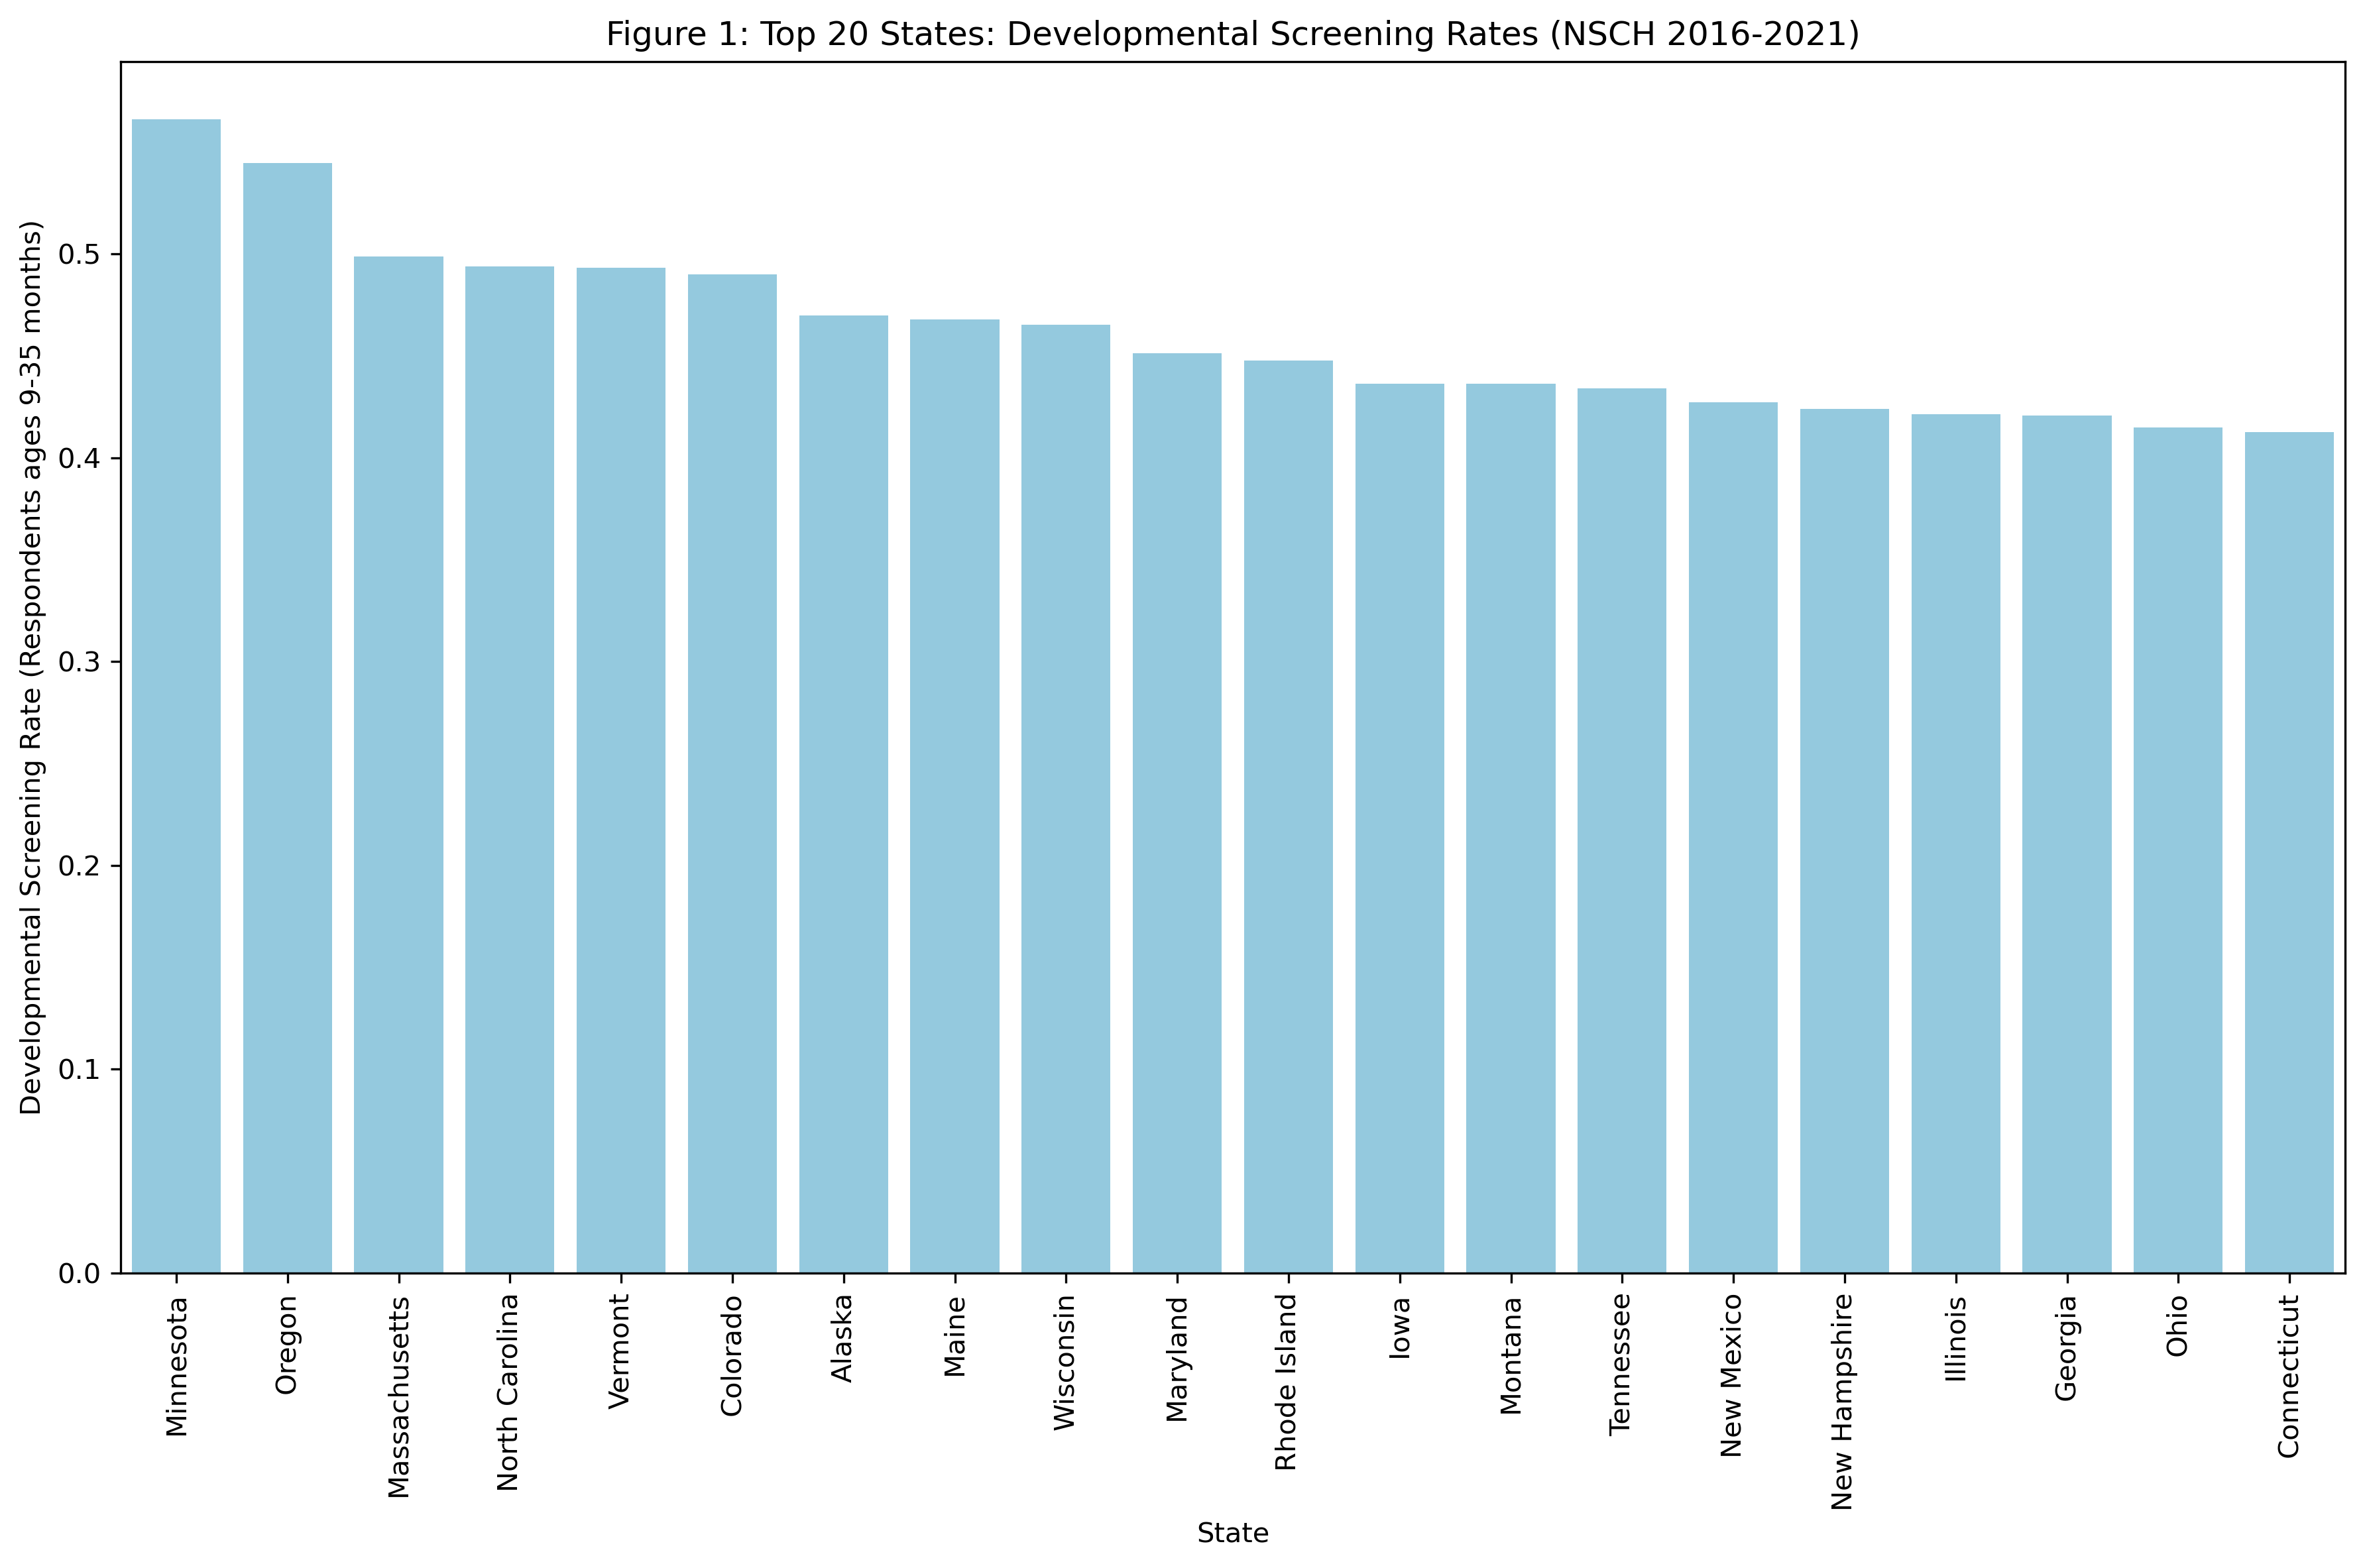
\includegraphics[width=0.8\textwidth]{images/Figure1_State_Screening_Rates.png}
\caption{State Developmental Screening Rates (2016-2020)}
\label{fig:state_rates}
\end{figure}

\begin{figure}[H]
\centering
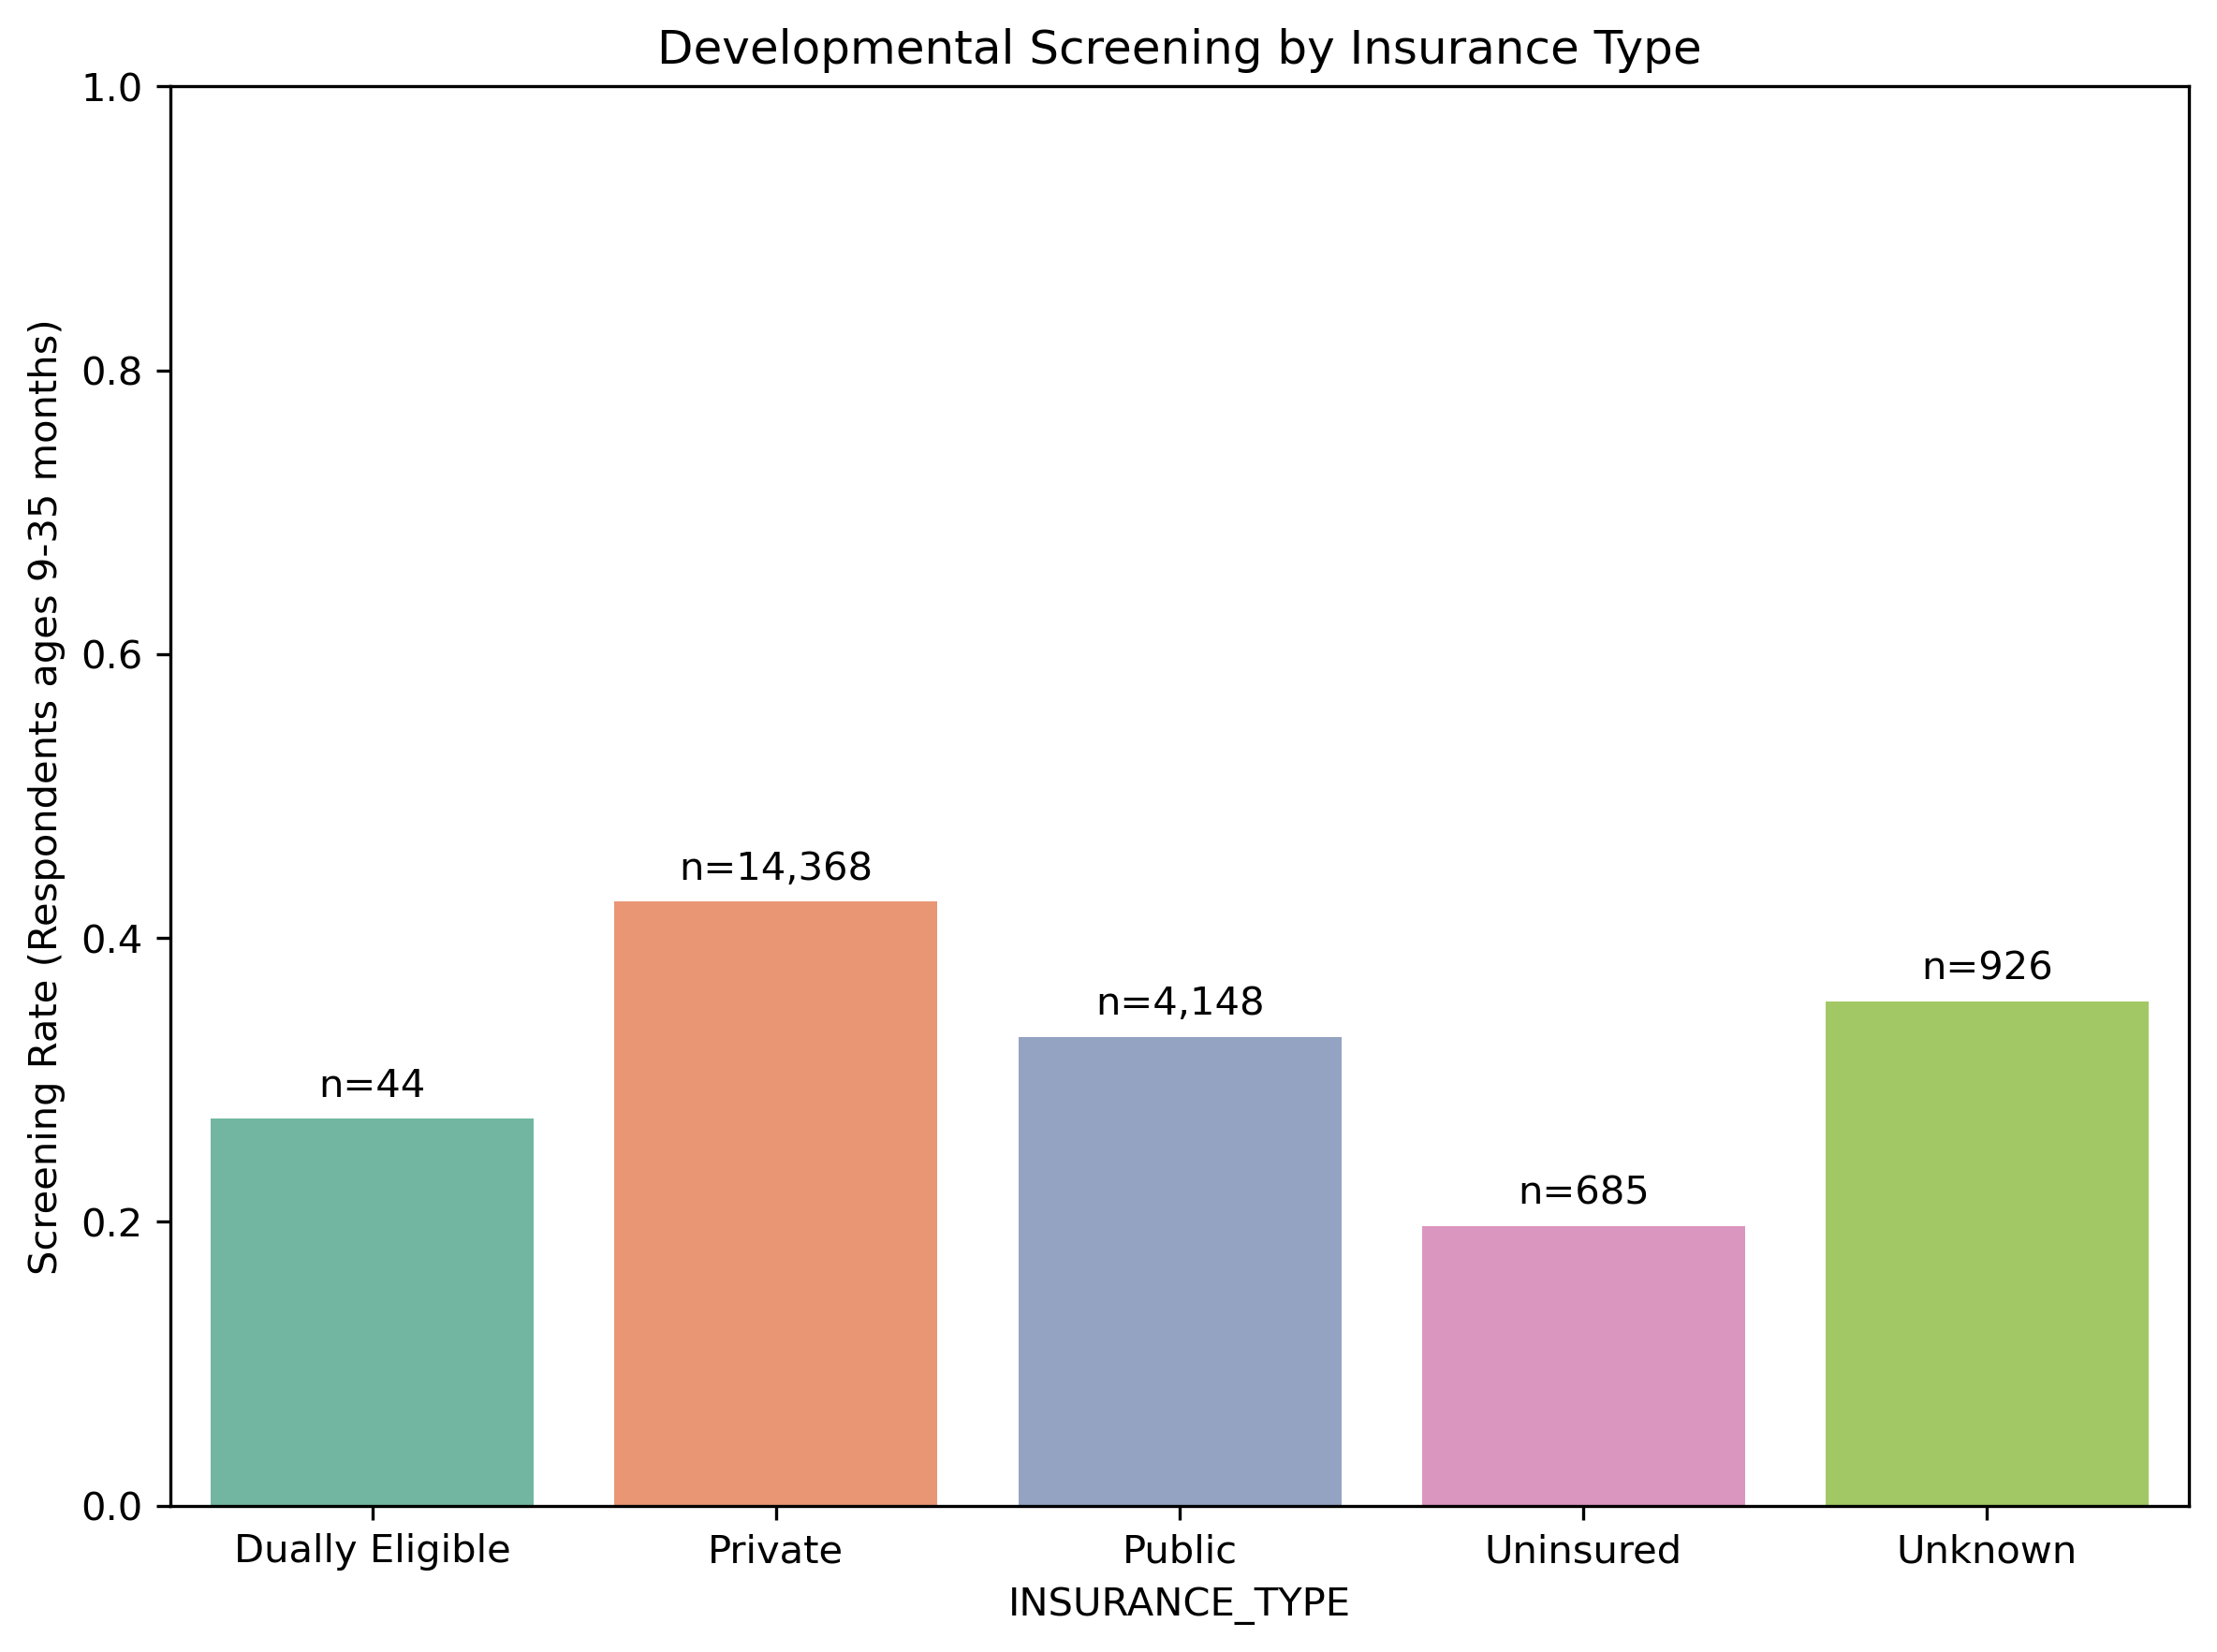
\includegraphics[width=0.8\textwidth]{images/Figure2_ScreenRatebyInsurance.png}
\caption{Developmental Screening Rates by Insurance Type (2016-2020)}
\label{fig:insurance_rates}
\end{figure}

\begin{figure}[H]
\centering
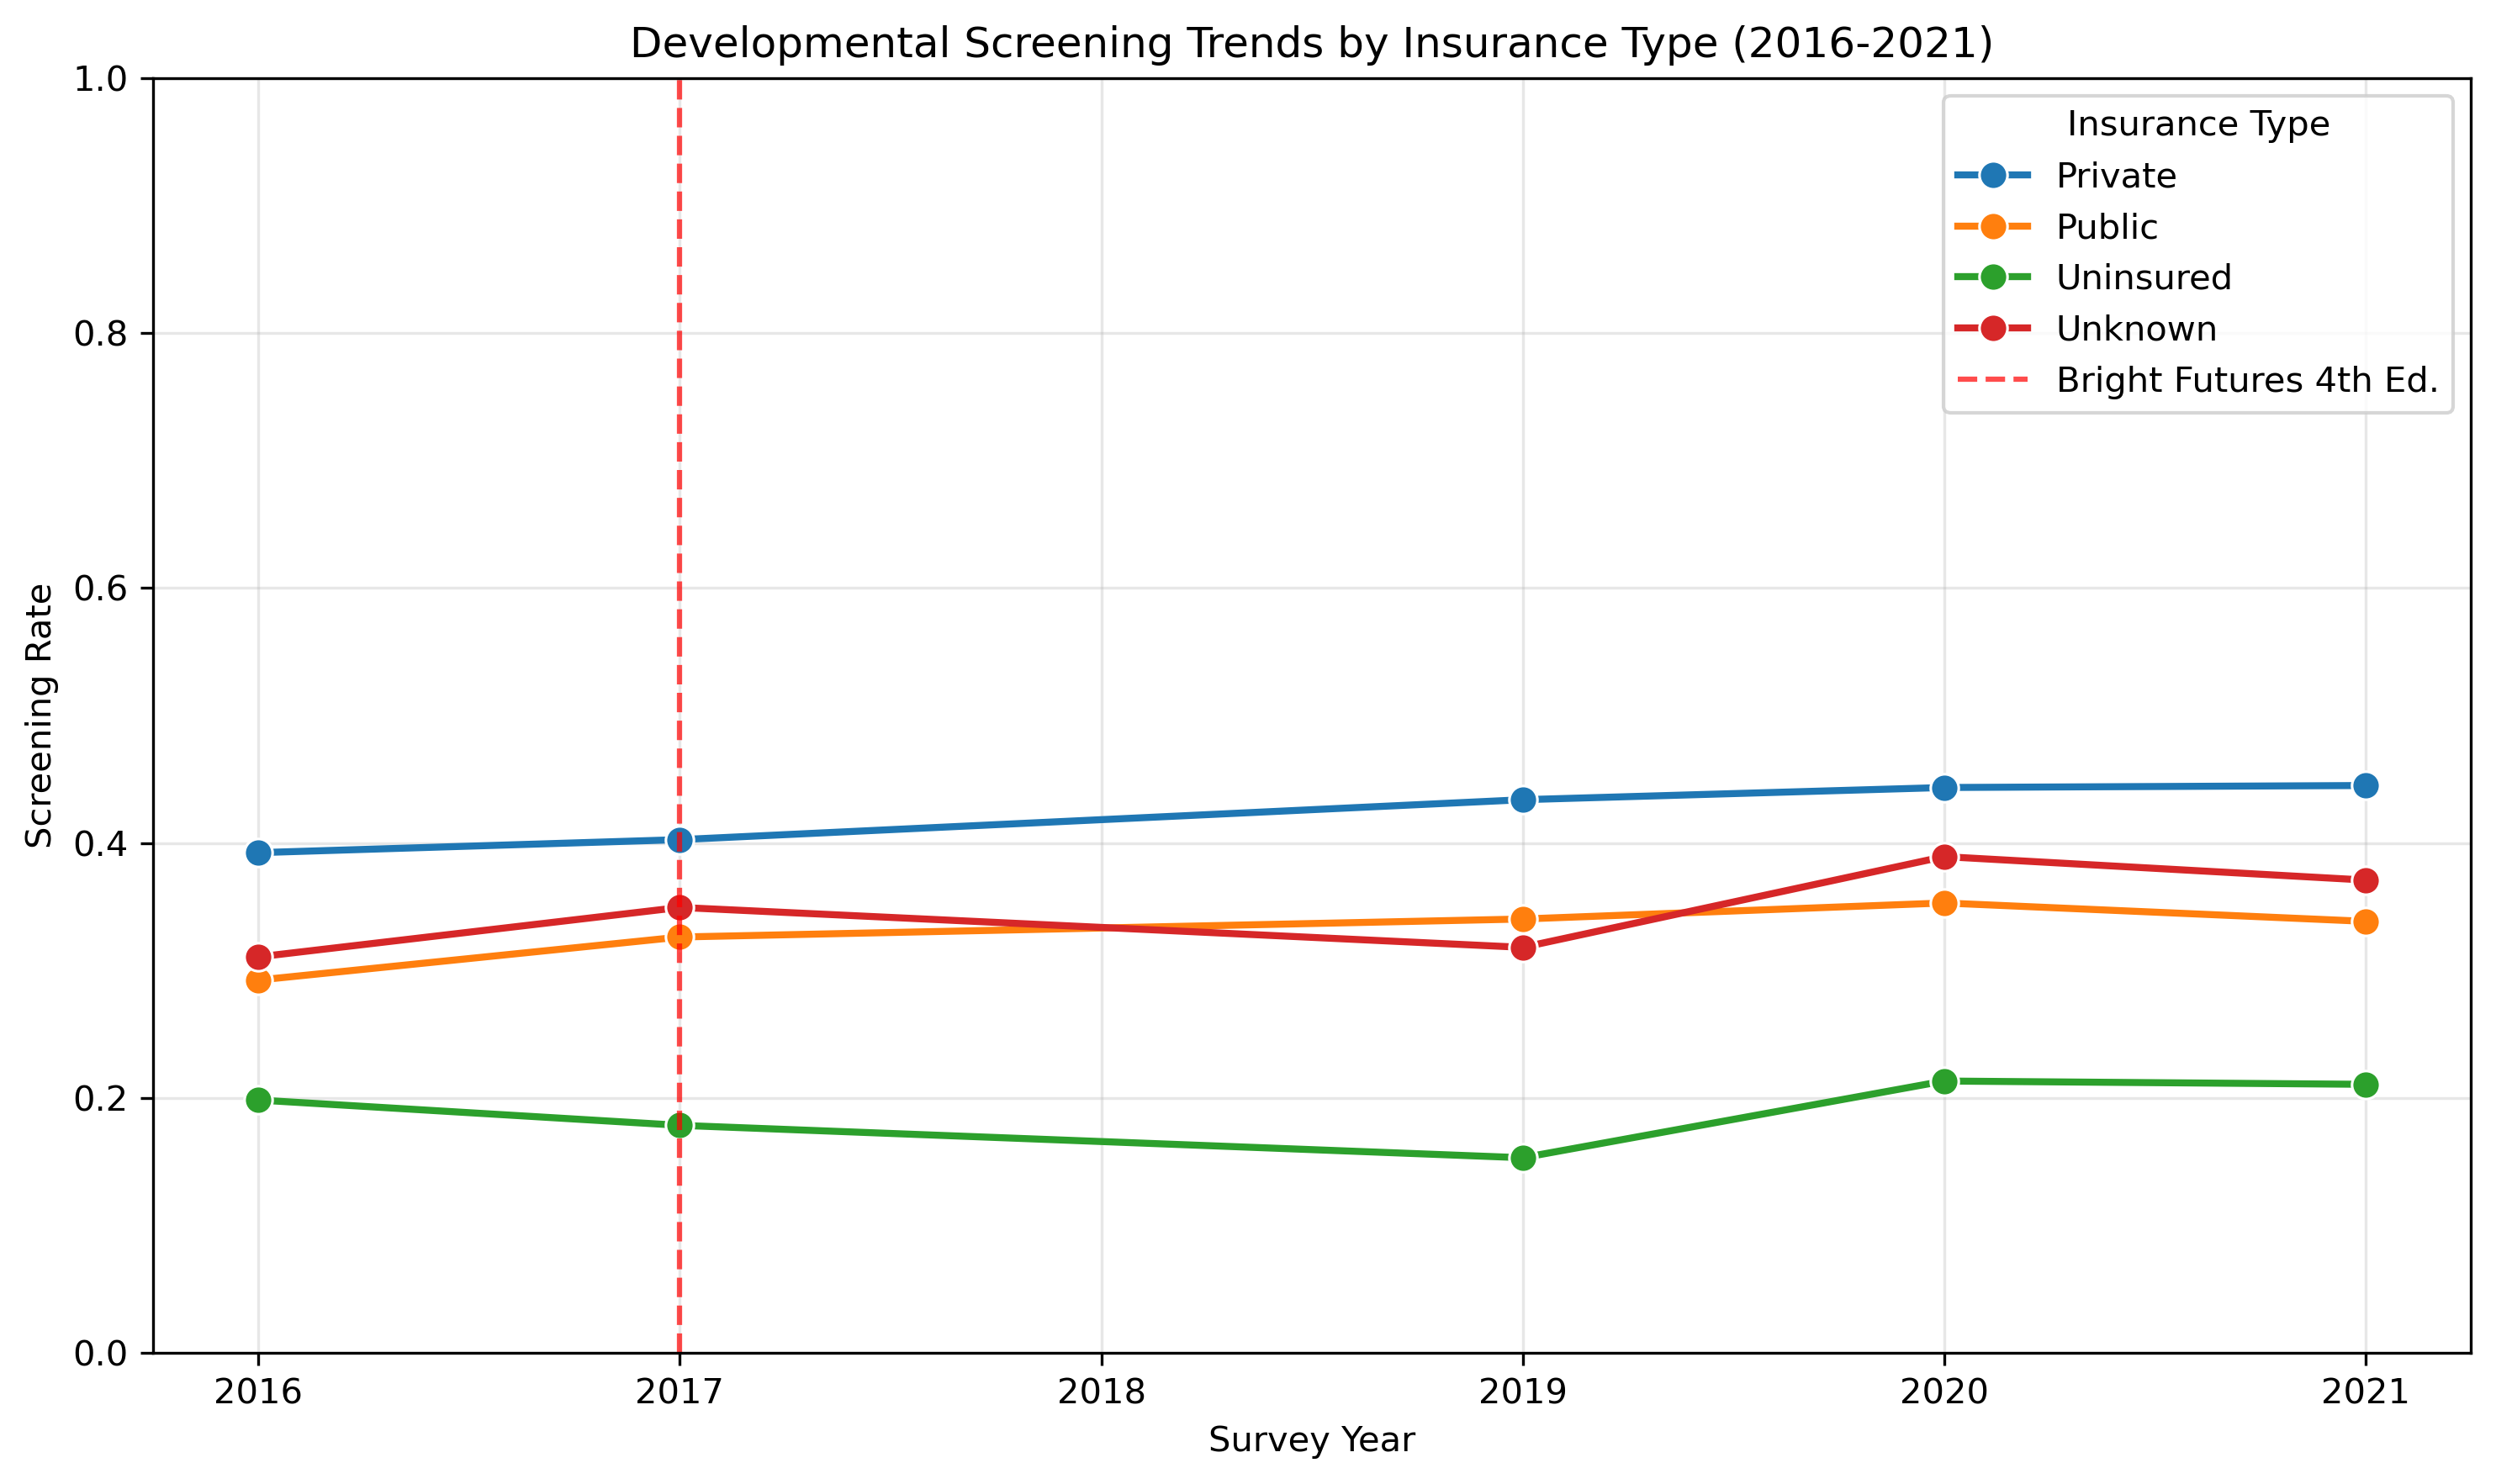
\includegraphics[width=0.8\textwidth]{images/Figure3_RD_BrightFutures2017.png}
\caption{Regression Discontinuity Design (2016-2020)}
\label{fig:rd_design}
\end{figure}

\begin{table}[!htbp] 
\centering
\caption{Regression Results: Developmental Screening}
\begin{adjustbox}{width=\textwidth,center}
\begin{tabular}{@{\extracolsep{5pt}}lccc}
\\[-1.8ex]\hline
\hline \\[-1.8ex]
& \multicolumn{3}{c}{\textit{Dependent variable: DEV\_SCREEN}} \\
\cline{2-4}
\\[-1.8ex] & \multicolumn{1}{c}{OLS} & \multicolumn{1}{c}{OLS + State FE} & \multicolumn{1}{c}{DiD} \\
\\[-1.8ex] & (1) & (2) & (3) \\
\hline \\[-1.8ex]
Age (Months) & -0.001$^{**}$ & -0.002$^{***}$ & -0.001$^{**}$ \\
& (0.001) & (0.001) & (0.001) \\
Black & -0.064$^{***}$ & -0.050$^{***}$ & -0.063$^{***}$ \\
& (0.014) & (0.015) & (0.014) \\
High Education & 0.126$^{***}$ & 0.116$^{***}$ & 0.123$^{***}$ \\
& (0.010) & (0.010) & (0.010) \\
Male & 0.005 & 0.003 & 0.005 \\
& (0.007) & (0.007) & (0.007) \\
Other Race & -0.035$^{***}$ & -0.038$^{***}$ & -0.036$^{***}$ \\
& (0.009) & (0.010) & (0.009) \\
Post-2017 & 0.044$^{***}$ & 0.042$^{***}$ & 0.044$^{***}$ \\
& (0.008) & (0.008) & (0.015) \\
Private Insurance & 0.105$^{***}$ & 0.102$^{***}$ & \\
& (0.012) & (0.012) & \\
Public Insurance & 0.053$^{***}$ & 0.052$^{***}$ & \\
& (0.013) & (0.013) & \\
Private Group & & & 0.068$^{***}$ \\
& & & (0.015) \\
DiD Effect & & & 0.001 \\
& & & (0.017) \\
Urban & 0.010 & 0.042$^{***}$ & 0.010 \\
& (0.007) & (0.010) & (0.007) \\
Intercept & 0.202$^{***}$ & 0.173$^{***}$ & 0.241$^{***}$ \\
& (0.021) & (0.033) & (0.021) \\
\hline \\[-1.8ex]
State Fixed Effects & No & Yes & No \\
Observations & 20,171 & 20,171 & 20,171 \\
$R^2$ & 0.020 & 0.043 & 0.019 \\
\hline
\hline \\[-1.8ex]
\textit{Note:} & \multicolumn{3}{r}{$^{*}$p$<$0.1; $^{**}$p$<$0.05; $^{***}$p$<$0.01} \\
\end{tabular}
\end{adjustbox}
\end{table}

\subsection{Unit Test Verification}

\begin{figure}[H]
\centering
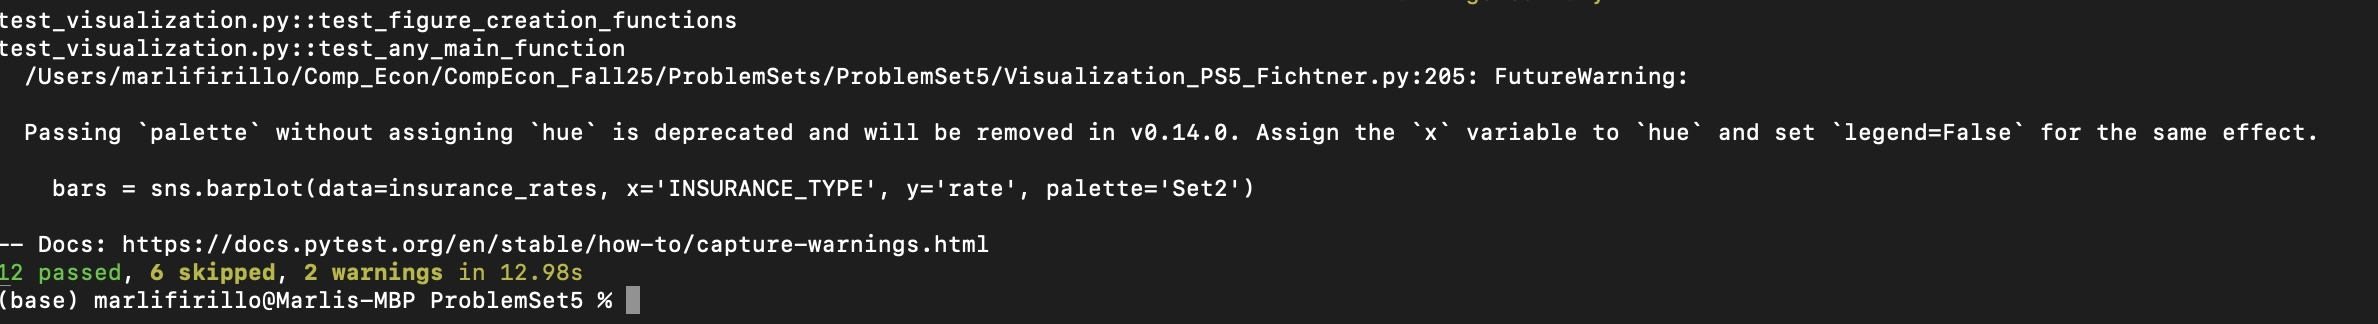
\includegraphics[width=0.8\textwidth]{images/TestVerify.jpg}
\caption{Unit Test Verification}
\label{fig:test_verification}
\end{figure}

\end{document}